\documentclass{dragonfly-report}\usepackage[]{graphicx}\usepackage[]{color}
%% maxwidth is the original width if it is less than linewidth
%% otherwise use linewidth (to make sure the graphics do not exceed the margin)
\makeatletter
\def\maxwidth{ %
  \ifdim\Gin@nat@width>\linewidth
    \linewidth
  \else
    \Gin@nat@width
  \fi
}
\makeatother

\definecolor{fgcolor}{rgb}{0.345, 0.345, 0.345}
\newcommand{\hlnum}[1]{\textcolor[rgb]{0.686,0.059,0.569}{#1}}%
\newcommand{\hlstr}[1]{\textcolor[rgb]{0.192,0.494,0.8}{#1}}%
\newcommand{\hlcom}[1]{\textcolor[rgb]{0.678,0.584,0.686}{\textit{#1}}}%
\newcommand{\hlopt}[1]{\textcolor[rgb]{0,0,0}{#1}}%
\newcommand{\hlstd}[1]{\textcolor[rgb]{0.345,0.345,0.345}{#1}}%
\newcommand{\hlkwa}[1]{\textcolor[rgb]{0.161,0.373,0.58}{\textbf{#1}}}%
\newcommand{\hlkwb}[1]{\textcolor[rgb]{0.69,0.353,0.396}{#1}}%
\newcommand{\hlkwc}[1]{\textcolor[rgb]{0.333,0.667,0.333}{#1}}%
\newcommand{\hlkwd}[1]{\textcolor[rgb]{0.737,0.353,0.396}{\textbf{#1}}}%

\usepackage{framed}
\makeatletter
\newenvironment{kframe}{%
 \def\at@end@of@kframe{}%
 \ifinner\ifhmode%
  \def\at@end@of@kframe{\end{minipage}}%
  \begin{minipage}{\columnwidth}%
 \fi\fi%
 \def\FrameCommand##1{\hskip\@totalleftmargin \hskip-\fboxsep
 \colorbox{shadecolor}{##1}\hskip-\fboxsep
     % There is no \\@totalrightmargin, so:
     \hskip-\linewidth \hskip-\@totalleftmargin \hskip\columnwidth}%
 \MakeFramed {\advance\hsize-\width
   \@totalleftmargin\z@ \linewidth\hsize
   \@setminipage}}%
 {\par\unskip\endMakeFramed%
 \at@end@of@kframe}
\makeatother

\definecolor{shadecolor}{rgb}{.97, .97, .97}
\definecolor{messagecolor}{rgb}{0, 0, 0}
\definecolor{warningcolor}{rgb}{1, 0, 1}
\definecolor{errorcolor}{rgb}{1, 0, 0}
\newenvironment{knitrout}{}{} % an empty environment to be redefined in TeX

\usepackage{alltt}

\usepackage{hyperref}

\title{Improving steepness priors in \emph{fishnets}}{Improving
  priors for the steepness of the stock-recruitment function within the R package \emph{fishnets}}

% Proposals require a subtitle which goes below the main title on the cover page. 
\subtitle{}
\author{Philipp Neubauer}

\addbibresource{steepness.bib}
\IfFileExists{upquote.sty}{\usepackage{upquote}}{}
\begin{document}
\maketitle

\section{Inferring steepness: available literature and estimation in the context of fishnets}

Steepness is generally defined as the fraction of recruitment from an unfished population ($R_0$) when the spawning stock biomass is at 20\% of its unfished (equilibrium) level ($B_0$). Given a functional form of the stock-recruit function $f$, steepness can be tied to the parameters of that function (at least in the case of the Ricker and Beverton-Holt (B-H) S-R functions), such that parameters of $f$ can be expressed in terms of steepness. However, depending on the form of $f$, the bounds on steepness are different: the Beverton-Holt S-R function admits steepness values in $[0.2;1]$ while the Ricker S-R function admits values between $0.2$ and infinity (i.e., recruitment can increase above $R_0$ at $0.2 B_0$). 

Given that the range of steepness varies among the B-H and Ricker S-R functions, steepness estimated from one S-R function is not directly applicable to the other, which posed a non-trivial problem for the development of a general purpose prior for steepness. Ideally, the steepness node should have a method for Ricker and B-H steepness. However, empirical approaches to the specification of prior distributions for steepness have generally focused on either one S-R model, with \citet{michielsens_2004_bayesian} being the exception. \citet{myers_1999_maximum} first provided estimates of B-H steepness for a large number of species and families based on Myers' S-R database. The estimates were simple transformations of the maximum lifetime reproductive rate, which was estimated from a meta-analysis using the Ricker S-R model across all stocks. \citet{michielsens_2004_bayesian} pointed out that fits of the Ricker and B-H functions lead to different estimates for the slope at the origin and different expectations for steepness. The direct transformation from Ricker model parameters to B-H steepness applied in Myers et al. 1999 therefore gives misleading (i.e., overly conservative) results.

Short of doing a new meta-analysis of steepness from the RAM legacy DB or other data source, \citet{myers_1999_maximum} was nevertheless considered an appropriate starting point for an empirical node as the reported estimates for the maximum lifetime reproductive rate make it possible to re-calculate the Ricker steepness (instead of the Beverton-Holt steepness reported in their paper). However, given the potentially strong selection bias in the study (for managed, VPA assessed stocks), it seemed less than ideal to use species or family level estimates from reported values directly. Rather, I attempted to use these estimates in combination with life-history to build a predictive model for steepness.

Theory suggests that recruitment variability and natural mortality M set the lower bounds for steepness \citep{he_2006_prior}. However, at low recruitment variability and M, there is little information about steepness in these parameters alone. Given an age structured model, Mangel et al. (2010; 2013) showed that steepness depends on growth, fecundity and mortality rates, and \citet{rose2001compensatory} provided evidence that empirical estimates of steepness follow expectations from life-history theory. Von Bertlanaffy growth and fecundity were therefore considered in addition to recruitment variability and natural mortality in the development of the empirical steepness node. Furthermore, given the complex relationships between life-history parameters and their constraints on steepness, a non-parametric node based on `brter` was considered the most practical start.

The biggest issue with an empirical node is that the only data that span a range of families and orders remains the somewhat outdated \citet{myers_1999_maximum}. The Myers dataset is the largest, but only gives unbiased estimates for the Ricker model steepness (i.e., after back-transforming and using equations in \citet{michielsens_2004_bayesian} to calculate Ricker steepness). \citet{shertzer2012spawner} obtain priors for demersal fish, but only provide an ad-hoc fit of truncated normal and beta distributions to estimates of steepness from stock assessments. Other datasets that provide more formally derived priors for steepness (e.g., \citet{michielsens_2004_bayesian}, \citet{dorn2002advice} and \citet{forrest2010hierarchical}) are too narrow to inform over broad enough a taxonomic range for an empirical node. Data from \citet{forrest2010hierarchical} were nevertheless included as estimates for US/Canada west-coast rockfish, in hope to obtain more robust estimates of empirical relationships with life-history parameters. However, the fundamental problem of inadequate sources of empirical estimates of steepness for the B-H function steepness means that it was be difficult to construct an empirical node for the B-H.

\section{An empirical steepness node}

\subsection{Data: a collated dataset for steepness}

Empirical estimates based on maximum lifetime reproductive rates were extracted from \citet{myers_1999_maximum}, and both mean B-H and Ricker steepness were recorded (the latter calculated using formulae in \citet{michielsens_2004_bayesian}), along with other parameters reported in \citet{myers_1999_maximum}. These data were augmented with data from \citet{forrest2010hierarchical} for \emph{Sebastes ssp.}. The combined dataset is available in the $\/data\/steepness$ directory as Myers\_et\_al\_steepness\_extended.csv. Data at the family level as also extracted and saved into Myers\_et\_al\_steepness\_families\_extended.csv.




A data node for steepness was implemented, such that 
\begin{knitrout}
\definecolor{shadecolor}{rgb}{0.969, 0.969, 0.969}\color{fgcolor}\begin{kframe}
\begin{alltt}
\hlcom{# Source in the package ----}

\hlkwd{source}\hlstd{(}\hlstr{'collate.R'}\hlstd{)}

\hlstd{steep} \hlkwb{<-} \hlstd{Steepness}\hlopt{$}\hlkwd{create}\hlstd{(}\hlstr{'./data/steepness'}\hlstd{)}
\hlkwd{head}\hlstd{(steep)}
\end{alltt}
\begin{verbatim}
##                species populations log_alpha_tilde SE_log_alpha_tilde
## 1    Harpodon nehereus           1            0.31               0.07
## 2 Alosa pseudoharengus           4            1.29               0.09
## 3    Alosa sapidissima           1            1.65               0.30
## 4  Brevoortia tyrannus           1            2.20               0.12
## 5     Alosa aestivalis           3            2.60               0.55
## 6  Brevoortia patronus           1            1.25               0.16
##   var_log_alpha_tilde exp_alpha_hat z_20 z_50 z_80 mean_R_z mean_BH_z
## 1                  NA           2.0   NA 0.34   NA     0.35      0.33
## 2                0.00           5.7   NA 0.59   NA     0.80      0.59
## 3                  NA          18.5   NA 0.82   NA     2.06      0.82
## 4                  NA          24.8   NA 0.86   NA     2.61      0.86
## 5                0.81          31.9 0.71 0.84 0.92     3.19      0.89
## 6                  NA           5.3   NA 0.57   NA     0.76      0.57
\end{verbatim}
\end{kframe}
\end{knitrout}

returns the data table. The table can then be merged with a fishbase data extract to pair empirical steepness estimates with life-history data. Note that the fishbase data is not restricted to species with $z$ estimates, rather the merge is, in SQL terms, a left join onto the fishbase data:

\begin{knitrout}
\definecolor{shadecolor}{rgb}{0.969, 0.969, 0.969}\color{fgcolor}\begin{kframe}
\begin{alltt}
\hlcom{# Load the Fishbase data}
\hlstd{fb} \hlkwb{<-} \hlstd{FishbaseWeb}\hlopt{$}\hlkwd{read}\hlstd{(}\hlstr{'data/fishbase-web'}\hlstd{)}
\hlcom{# Limit to the 7940 with both k and linf}
\hlstd{fb} \hlkwb{<-} \hlkwd{subset}\hlstd{(fb,}\hlopt{!}\hlkwd{is.na}\hlstd{(k)} \hlopt{& !}\hlkwd{is.na}\hlstd{(linf))}
\hlcom{# An an id column for indexing later}
\hlstd{fb}\hlopt{$}\hlstd{id} \hlkwb{<-} \hlnum{1}\hlopt{:}\hlkwd{nrow}\hlstd{(fb)}
\hlcom{# Add a dummy row for helping with predictor nodes}
\hlcom{# that need to have at least two predictors}
\hlstd{fb}\hlopt{$}\hlstd{dummy} \hlkwb{<-} \hlnum{1.0}

\hlcom{# merge with steepness data}
\hlstd{steep_merged} \hlkwb{<-} \hlstd{Steepness}\hlopt{$}\hlkwd{merge}\hlstd{(steep,fb)}

\hlkwd{head}\hlstd{(steep_merged)}
\end{alltt}
\begin{verbatim}
##               species populations log_alpha_tilde SE_log_alpha_tilde
## 1 Abbottina rivularis          NA              NA                 NA
## 2      Ablennes hians          NA              NA                 NA
## 3       Abramis brama          NA              NA                 NA
## 4       Abramis brama          NA              NA                 NA
## 5       Abramis brama          NA              NA                 NA
## 6       Abramis brama          NA              NA                 NA
##   var_log_alpha_tilde exp_alpha_hat z_20 z_50 z_80 mean_R_z mean_BH_z
## 1                  NA            NA   NA   NA   NA       NA        NA
## 2                  NA            NA   NA   NA   NA       NA        NA
## 3                  NA            NA   NA   NA   NA       NA        NA
## 4                  NA            NA   NA   NA   NA       NA        NA
## 5                  NA            NA   NA   NA   NA       NA        NA
## 6                  NA            NA   NA   NA   NA       NA        NA
##           order     country sex     genus     family       swimmode ltype
## 1 Cypriniformes Russian Fed   U Abbottina Cyprinidae             na    NG
## 2  Beloniformes       India   U  Ablennes  Belonidae             na    FL
## 3 Cypriniformes      Poland   U   Abramis Cyprinidae subcarangiform    TL
## 4 Cypriniformes Former USSR   U   Abramis Cyprinidae subcarangiform    TL
## 5 Cypriniformes Russian Fed   U   Abramis Cyprinidae subcarangiform    TL
## 6 Cypriniformes     Germany   U   Abramis Cyprinidae subcarangiform    TL
##    linf    k t0    m temp lmat lmatmin lmatmax amat amatmin amatmax
## 1  15.8 0.30  0   NA   NA   NA       4     5.0    1      NA      NA
## 2 123.0 0.61  0   NA 27.0   NA      NA      NA   NA      NA      NA
## 3  91.4 0.09  0   NA   NA   NA      25    32.5   NA      NA      NA
## 4 109.0 0.10  0   NA  6.5   NA      NA      NA   NA       3       5
## 5  42.0 0.23  0 0.17  8.0   NA      NA      NA   NA      NA      NA
## 6  61.8 0.07  0   NA  8.3   NA      NA      NA   NA      NA      NA
##         a      b trophic      diet                       feeding
## 1      NA     NA      NA      <NA>                          <NA>
## 2 0.00036 3.3220    4.50 secondary hunting macrofauna (predator)
## 3 0.01763 3.0825    3.15 secondary hunting macrofauna (predator)
## 4 0.02500 3.0000    3.15 secondary hunting macrofauna (predator)
## 5 0.01940 3.0365    3.15 secondary hunting macrofauna (predator)
## 6      NA     NA    3.15 secondary hunting macrofauna (predator)
##             habit     migration depthmin depthmax fecundmin fecundmax
## 1   benthopelagic    freshwater       NA       NA        NA        NA
## 2 reef-associated oceanodromous        0        3        NA        NA
## 3   benthopelagic potamodromous        1       NA     20800    309600
## 4   benthopelagic potamodromous        1       NA     20800    309600
## 5   benthopelagic potamodromous        1       NA     20800    309600
## 6   benthopelagic potamodromous        1       NA     20800    309600
##   fecundity          class     lmax amax   id dummy
## 1        NA Actinopterygii       NA   NA 7728     1
## 2        NA Actinopterygii       NA   NA 3229     1
## 3    759847 Actinopterygii 48.33333   NA 1813     1
## 4    759847 Actinopterygii 48.33333   NA 1814     1
## 5    759847 Actinopterygii 48.33333   NA 1815     1
## 6    759847 Actinopterygii 48.33333   NA 1816     1
\end{verbatim}
\end{kframe}
\end{knitrout}

In order to set up a fishnet that that extracts empirical relationships between steepness and life-history, the merged fishbase/steepness data was aggregated at species level to avoid multiple, possibly contradictory, life-history correlates with steepness. Geometric means were used to aggregate life-history parameters, under thew assumption that most follow log-normal distributions.

\begin{knitrout}
\definecolor{shadecolor}{rgb}{0.969, 0.969, 0.969}\color{fgcolor}\begin{kframe}
\begin{alltt}
\hlkwd{require}\hlstd{(dplyr)}

\hlcom{# geometric mean}
\hlstd{gmean} \hlkwb{<-} \hlkwa{function}\hlstd{(}\hlkwc{x}\hlstd{)} \hlkwd{exp}\hlstd{(}\hlkwd{mean}\hlstd{(}\hlkwd{log}\hlstd{(x),}\hlkwc{na.rm}\hlstd{=T))}

\hlcom{# reduce dataset; gometric means for paramters by species}
\hlstd{steep_reduced} \hlkwb{<-} \hlstd{steep_merged} \hlopt
  \hlkwd{select}\hlstd{(species, genus, family, class, order, mean_BH_z, linf, m, fecundity, trophic, lmat, lmax , k, amax, habit, trophic, depthmax)} \hlopt
  \hlkwd{group_by}\hlstd{(order,class,genus,family,species)} \hlopt
  \hlkwd{summarise}\hlstd{(}\hlkwc{mean_BH_z} \hlstd{=} \hlkwd{unique}\hlstd{(mean_BH_z),}
            \hlkwc{habit} \hlstd{=} \hlkwd{unique}\hlstd{(habit),}
            \hlkwc{trophic} \hlstd{=} \hlkwd{gmean}\hlstd{(trophic),}
            \hlkwc{linf} \hlstd{=} \hlkwd{gmean}\hlstd{(linf),}
            \hlkwc{m} \hlstd{=} \hlkwd{gmean}\hlstd{(m),}
            \hlkwc{depthmax} \hlstd{=} \hlkwd{gmean}\hlstd{(depthmax),}
            \hlkwc{fecundity} \hlstd{=} \hlkwd{gmean}\hlstd{(fecundity),}
            \hlkwc{trophic} \hlstd{=} \hlkwd{gmean}\hlstd{(trophic),}
            \hlkwc{lmax} \hlstd{=} \hlkwd{gmean}\hlstd{(lmax),}
            \hlkwc{lmat} \hlstd{=} \hlkwd{gmean}\hlstd{(lmat),}
            \hlkwc{k} \hlstd{=} \hlkwd{gmean}\hlstd{(k),}
            \hlkwc{amax} \hlstd{=} \hlkwd{gmean}\hlstd{(amax),}
            \hlkwc{recsigma} \hlstd{=} \hlnum{NA}\hlstd{)} \hlopt
  \hlkwd{ungroup}\hlstd{()} \hlopt
  \hlkwd{data.frame}\hlstd{()}
\end{alltt}
\end{kframe}
\end{knitrout}

\subsection{A Bayesian empirical node to avoid overfitting}

An initial attempot at defining a fishnet based on previously available nodes (brter: boosted regression trees; svmer: support vector machines; glmer: generalized linear models) suggested that overfitting of empirical relationships might be interferring with predictive power of the nodes. To investigate this potential problem, I implemented a Bayesian node based on the \href{http://www.r-inla.org/}{INLA} package in R. Fully Bayesian methods are less prone to overfitting, and the INLA approach, based on laplacian approximations, allows for fast parameter estiamtion in linear and linear mixed models. The resulting node, called \emph{bayser}, uses the same formula syntax as previous empirical nodes, with additional option to estiamte random effects with the $f(effect, 'iid')$ syntax (e.g., f(family,model="iid") for a family level random effect). This option should facilitate the use of taxonomic information in empirical nodes, whereas the use of taxonomy as a fixed effect frequently leads to overfitting. The \emph{bayser} node comes with $fit$, $sample$, $predict$ and $tune$ methods:

\begin{knitrout}
\definecolor{shadecolor}{rgb}{0.969, 0.969, 0.969}\color{fgcolor}\begin{kframe}
\begin{alltt}
\hlstd{linf} \hlkwb{=} \hlkwd{Bayser}\hlstd{(}\hlkwd{log}\hlstd{(linf)} \hlopt{~} \hlkwd{f}\hlstd{(family,}\hlkwc{model}\hlstd{=}\hlstr{"iid"}\hlstd{)}\hlopt{+}\hlkwd{f}\hlstd{(order,}\hlkwc{model}\hlstd{=}\hlstr{"iid"}\hlstd{)}\hlopt{+}\hlkwd{log}\hlstd{(lmax)}\hlopt{+}\hlstd{habit,exp)}
\hlcom{# fitting to data}
\hlstd{linf}\hlopt{$}\hlkwd{fit}\hlstd{(steep_reduced[}\hlnum{1}\hlopt{:}\hlnum{1500}\hlstd{,])}

\hlcom{# predicting onto new data}
\hlstd{example_predictions} \hlkwb{<-} \hlstd{linf}\hlopt{$}\hlkwd{predict}\hlstd{(steep_reduced[}\hlnum{1501}\hlopt{:}\hlkwd{nrow}\hlstd{(steep_reduced),])}

\hlstd{predict_df} \hlkwb{<-} \hlkwd{data.frame}\hlstd{(}\hlkwc{bayser} \hlstd{= example_predictions[}\hlopt{!}\hlkwd{is.na}\hlstd{(steep_reduced}\hlopt{$}\hlstd{lmax[}\hlnum{1501}\hlopt{:}\hlkwd{nrow}\hlstd{(steep_reduced)])],} \hlkwc{observed} \hlstd{= steep_reduced[}\hlnum{1501}\hlopt{:}\hlkwd{nrow}\hlstd{(steep_reduced),}\hlstr{'linf'}\hlstd{][}\hlopt{!}\hlkwd{is.na}\hlstd{(steep_reduced}\hlopt{$}\hlstd{lmax[}\hlnum{1501}\hlopt{:}\hlkwd{nrow}\hlstd{(steep_reduced)])])}

\hlstd{linf_brter} \hlkwb{=} \hlkwd{Brter}\hlstd{(}\hlkwd{log}\hlstd{(linf)} \hlopt{~} \hlstd{family} \hlopt{+} \hlstd{order}\hlopt{+} \hlkwd{log}\hlstd{(lmax)}\hlopt{+}\hlstd{habit,exp)}
\hlcom{# fitting to data}
\hlstd{linf_brter}\hlopt{$}\hlkwd{fit}\hlstd{(steep_reduced[}\hlnum{1}\hlopt{:}\hlnum{1500}\hlstd{,])}
\end{alltt}
\begin{verbatim}
## [1] fitting gbm model with a fixed number of 2000 trees for log(linf)
## [1] total deviance = 228.52
## [1] residual deviance = 19.65
## predictors: family order log(lmax) habit
\end{verbatim}
\begin{alltt}
\hlcom{# predicting onto new data}
\hlstd{example_predictions_brter} \hlkwb{<-} \hlstd{linf_brter}\hlopt{$}\hlkwd{predict}\hlstd{(steep_reduced[}\hlnum{1501}\hlopt{:}\hlkwd{nrow}\hlstd{(steep_reduced),])}

\hlstd{predict_df} \hlkwb{<-} \hlstd{reshape2::}\hlkwd{melt}\hlstd{(}\hlkwd{data.frame}\hlstd{(}\hlkwc{brter} \hlstd{= example_predictions_brter[}\hlopt{!}\hlkwd{is.na}\hlstd{(steep_reduced}\hlopt{$}\hlstd{lmax[}\hlnum{1501}\hlopt{:}\hlkwd{nrow}\hlstd{(steep_reduced)])],predict_df),}\hlkwc{id.vars} \hlstd{=} \hlkwd{c}\hlstd{(}\hlstr{'observed'}\hlstd{))}
\end{alltt}
\end{kframe}
\end{knitrout}

\begin{knitrout}
\definecolor{shadecolor}{rgb}{0.969, 0.969, 0.969}\color{fgcolor}\begin{kframe}
\begin{alltt}
\hlkwd{require}\hlstd{(ggplot2)}

\hlkwd{ggplot}\hlstd{(predict_df)} \hlopt{+}
  \hlkwd{geom_point}\hlstd{(}\hlkwd{aes}\hlstd{(}\hlkwc{y} \hlstd{= value,} \hlkwc{x} \hlstd{= observed,} \hlkwc{col} \hlstd{= variable))} \hlopt{+}
  \hlkwd{geom_abline}\hlstd{(}\hlkwc{slope}\hlstd{=}\hlnum{1}\hlstd{,} \hlkwc{intercept}\hlstd{=}\hlnum{0}\hlstd{)} \hlopt{+}
  \hlkwd{theme_bw}\hlstd{()} \hlopt{+}
  \hlkwd{xlab}\hlstd{(}\hlstr{'Data'}\hlstd{)} \hlopt{+}
  \hlkwd{ylab}\hlstd{(}\hlstr{'Prediction'}\hlstd{)} \hlopt{+}
  \hlkwd{scale_colour_discrete}\hlstd{(}\hlstr{'Method'}\hlstd{)}
\end{alltt}
\end{kframe}\begin{figure}[]


{\centering 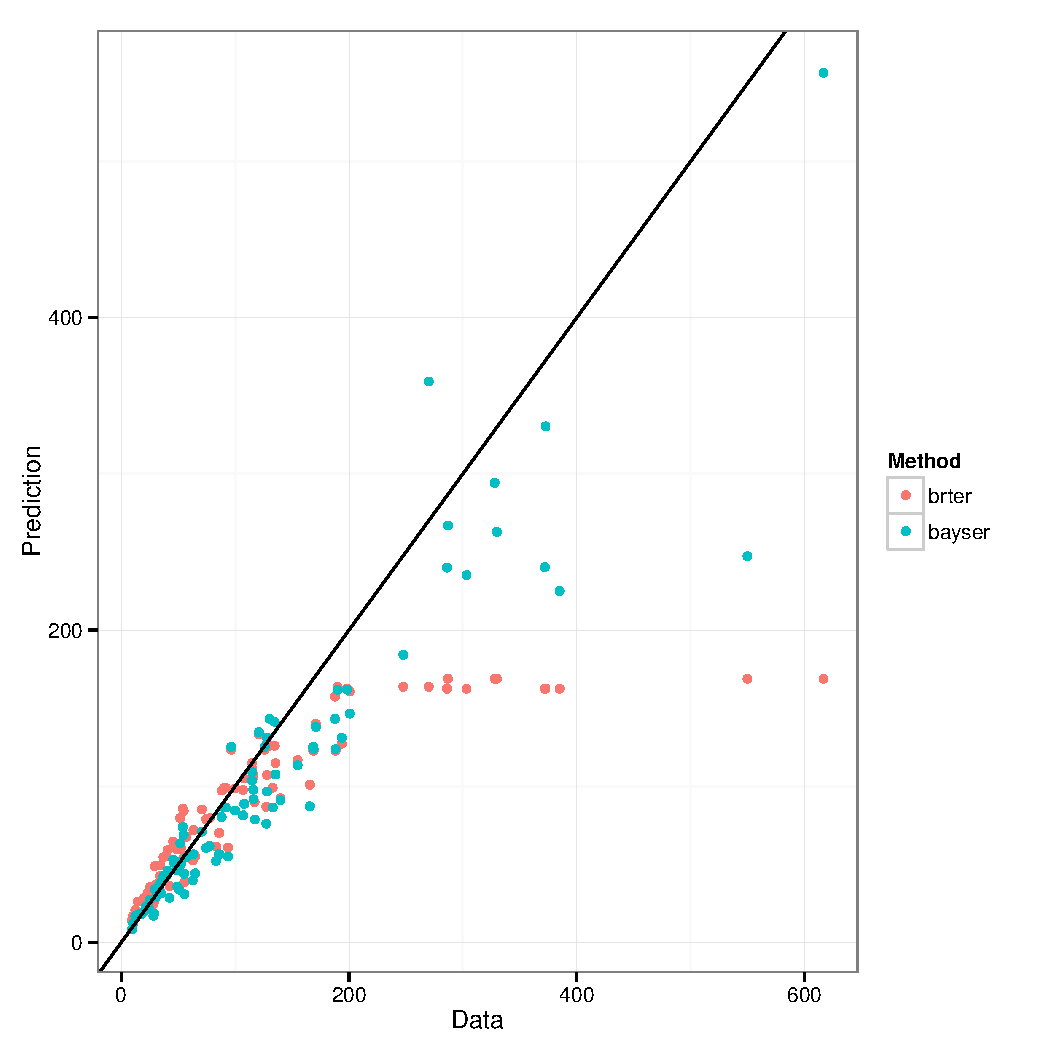
\includegraphics[width=3in,height=3 in]{figure/unnamed-chunk-2-1} 

}

\caption[Example predictions for linf as a function of lmax and taxonomy on a subset of fishbase data, showing that the predictive power in Bayser can be superior to that of Brter when taxonomy is used as a predictor]{Example predictions for linf as a function of lmax and taxonomy on a subset of fishbase data, showing that the predictive power in Bayser can be superior to that of Brter when taxonomy is used as a predictor.\label{fig:unnamed-chunk-2}}
\end{figure}


\end{knitrout}


\subsection{Sequential imputing of data in fishnets}

In the $Bayser$ example above, $linf$ depends on $lmax$ in an empirical node. The relationship can only be estiamted for data rows (i.e.,species) with data for both traits. For more complex life history interactions, missing data for the combination of covariantes in the model can strongly influence the total number of species for which the relationship can be estriamted. For example, one species may not have a reported von Bertlanaffy k, while another species may have k but no estiamte of fecundity. Neither row could be inlcuded in a node like steepness, which may dpend on both factors. In the case of steepness, only 46 empirical estiamtes at the species level are available from the dataset described above, and missing values dramatically reduce the number of covariates taht could be used to construct an empirical node for steepness.

To obtain more data for complex empirical relationships, I implemented an option within the generic $fit$ method of a fishnet, which allows data to be sequentially imputed. Thus, if linf depends on lmax, and k in turn depends on linf, then linf could be imputed for species with missing linf based on the node relating it to lmax. This allows k to be estiamted for species with data for lamx and missing data for linf. The imputation naturally relies on a linearly evolving net, where relationships depend on  values imputed at lower level nodes. The option can be turned on using $impute = TRUE$ when fitting a fishnet (see the steepness node fitting below).

\subsection{The empirical steepness node: fishing for predictive power}

The empirical fishnet node to estiamte steepness was embedded in a larger fishnet that aimed to build a covariate set (using the $impute~=~T$ option).

\begin{knitrout}
\definecolor{shadecolor}{rgb}{0.969, 0.969, 0.969}\color{fgcolor}\begin{kframe}
\begin{alltt}
\hlcom{# build a net for steepnes. Use Bayesian nodes in an attempt to not overfit (i.e., to get better predictive power)}
\hlcom{# transformations are defined for Beverton-Holt S-R parameters to map steepness onto the real line and back.}

\hlstd{logit} \hlkwb{<-} \hlkwa{function}\hlstd{(}\hlkwc{x}\hlstd{)} \hlkwd{log}\hlstd{(x}\hlopt{/}\hlstd{(}\hlnum{1}\hlopt{-}\hlstd{x))}
\hlstd{logit_inv} \hlkwb{<-} \hlkwa{function}\hlstd{(}\hlkwc{xt}\hlstd{)} \hlnum{1}\hlopt{/}\hlstd{(}\hlnum{1} \hlopt{+} \hlkwd{exp}\hlstd{(}\hlopt{-}\hlstd{xt))}
\hlstd{BH_tr} \hlkwb{<-} \hlkwa{function}\hlstd{(}\hlkwc{h}\hlstd{) h}\hlopt{/}\hlnum{0.8}\hlopt{-}\hlnum{0.25}
\hlstd{BH_tr_inv} \hlkwb{<-} \hlkwa{function}\hlstd{(}\hlkwc{ht}\hlstd{) (ht}\hlopt{+}\hlnum{0.25}\hlstd{)}\hlopt{*}\hlnum{0.8}
\hlstd{logit_BH} \hlkwb{<-} \hlkwa{function}\hlstd{(}\hlkwc{h}\hlstd{)} \hlkwd{logit}\hlstd{(}\hlkwd{BH_tr}\hlstd{(h))}
\hlstd{logit_BH_inv} \hlkwb{<-} \hlkwa{function}\hlstd{(}\hlkwc{ht}\hlstd{)} \hlkwd{BH_tr_inv}\hlstd{(}\hlkwd{logit_inv}\hlstd{(ht))}

\hlstd{BH_net} \hlkwb{<-} \hlkwd{Fishnet}\hlstd{(}
  \hlkwc{species}   \hlstd{=} \hlkwd{SpeciesRandom}\hlstd{(),}
  \hlkwc{genus}     \hlstd{=} \hlkwd{GenusParser}\hlstd{(),}
  \hlkwc{family}    \hlstd{=} \hlkwd{FamilyLookupper}\hlstd{(),}
  \hlkwc{order}     \hlstd{=} \hlkwd{OrderLookupper}\hlstd{(),}
  \hlkwc{class}     \hlstd{=} \hlkwd{ClassLookupper}\hlstd{(),}

  \hlkwc{habit}     \hlstd{=} \hlkwd{TaxonomicImputer}\hlstd{(}\hlstr{'habit'}\hlstd{),}
  \hlkwc{depthmax}  \hlstd{=} \hlkwd{TaxonomicImputer}\hlstd{(}\hlstr{'depthmax'}\hlstd{,}\hlkwd{c}\hlstd{(log,exp),}\hlnum{5}\hlstd{),}
  \hlkwc{trophic}   \hlstd{=} \hlkwd{TaxonomicImputer}\hlstd{(}\hlstr{'trophic'}\hlstd{,}\hlkwd{c}\hlstd{(log,exp),}\hlnum{3}\hlstd{),}
  \hlkwc{lmax}      \hlstd{=} \hlkwd{TaxonomicImputer}\hlstd{(}\hlstr{'lmax'}\hlstd{,}\hlkwd{c}\hlstd{(log,exp),}\hlnum{5}\hlstd{),}
  \hlkwc{amax}      \hlstd{=} \hlkwd{TaxonomicImputer}\hlstd{(}\hlstr{'amax'}\hlstd{,}\hlkwd{c}\hlstd{(log,exp),}\hlnum{5}\hlstd{),}

  \hlkwc{linf}      \hlstd{=} \hlkwd{Bayser}\hlstd{(}\hlkwd{log}\hlstd{(linf)} \hlopt{~} \hlkwd{f}\hlstd{(family,}\hlkwc{model}\hlstd{=}\hlstr{"iid"}\hlstd{)}\hlopt{+}\hlkwd{f}\hlstd{(class,}\hlkwc{model}\hlstd{=}\hlstr{"iid"}\hlstd{)}\hlopt{+}\hlkwd{log}\hlstd{(lmax),exp),}
  \hlkwc{fecundity} \hlstd{=} \hlkwd{Bayser}\hlstd{(}\hlkwd{log}\hlstd{(fecundity)} \hlopt{~} \hlkwd{f}\hlstd{(family,}\hlkwc{model}\hlstd{=}\hlstr{"iid"}\hlstd{)}\hlopt{+}\hlkwd{f}\hlstd{(class,}\hlkwc{model}\hlstd{=}\hlstr{"iid"}\hlstd{)} \hlopt{+} \hlkwd{log}\hlstd{(linf)} \hlopt{+} \hlkwd{log}\hlstd{(depthmax),exp),}
  \hlkwc{k}         \hlstd{=} \hlkwd{Bayser}\hlstd{(}\hlkwd{log}\hlstd{(k)} \hlopt{~} \hlkwd{f}\hlstd{(family,}\hlkwc{model}\hlstd{=}\hlstr{"iid"}\hlstd{)} \hlopt{+} \hlkwd{log}\hlstd{(linf)} \hlopt{+} \hlkwd{f}\hlstd{(habit,}\hlkwc{model}\hlstd{=}\hlstr{"iid"}\hlstd{)} \hlopt{+} \hlkwd{log}\hlstd{(depthmax),exp),}
  \hlkwc{m}         \hlstd{=} \hlkwd{Bayser}\hlstd{(}\hlkwd{log}\hlstd{(m)} \hlopt{~} \hlkwd{f}\hlstd{(family,}\hlkwc{model}\hlstd{=}\hlstr{"iid"}\hlstd{)}\hlopt{+}\hlkwd{f}\hlstd{(class,}\hlkwc{model}\hlstd{=}\hlstr{"iid"}\hlstd{)}\hlopt{+}\hlkwd{log}\hlstd{(k)}\hlopt{+}\hlkwd{log}\hlstd{(linf)}\hlopt{+}\hlkwd{f}\hlstd{(habit,}\hlkwc{model}\hlstd{=}\hlstr{"iid"}\hlstd{)}\hlopt{+}\hlkwd{log}\hlstd{(depthmax)}\hlopt{+}\hlstd{trophic,exp),}
  \hlkwc{lmat}      \hlstd{=} \hlkwd{Bayser}\hlstd{(}\hlkwd{log}\hlstd{(lmat)} \hlopt{~} \hlkwd{f}\hlstd{(family,}\hlkwc{model}\hlstd{=}\hlstr{"iid"}\hlstd{)}\hlopt{+}\hlkwd{log}\hlstd{(k)}\hlopt{+}\hlkwd{log}\hlstd{(linf)}\hlopt{+}\hlkwd{f}\hlstd{(habit,}\hlkwc{model}\hlstd{=}\hlstr{"iid"}\hlstd{)}\hlopt{+}\hlkwd{log}\hlstd{(depthmax),exp),}
  \hlkwc{recsigma}  \hlstd{=} \hlkwd{RecsigmaThorsonEtAl2014}\hlstd{(),}
  \hlkwc{mean_BH_z} \hlstd{=} \hlkwd{Brter}\hlstd{(}\hlkwd{logit_BH}\hlstd{(mean_BH_z)} \hlopt{~}  \hlstd{habit} \hlopt{+} \hlkwd{log}\hlstd{(linf)} \hlopt{+} \hlkwd{log}\hlstd{(k)} \hlopt{+} \hlkwd{log}\hlstd{(m)}\hlopt{+} \hlkwd{log}\hlstd{(fecundity)} \hlopt{+}\hlstd{recsigma} \hlopt{+} \hlstd{trophic}\hlopt{+}\hlkwd{log}\hlstd{(depthmax),}\hlkwc{transform} \hlstd{= logit_BH_inv,}\hlkwc{ntrees} \hlstd{=}\hlnum{3500}\hlstd{,}\hlkwc{bag.fraction}\hlstd{=}\hlnum{0.9}\hlstd{)}

\hlstd{)}

\hlcom{# fit the BH_et to the summarised fishbase data}
\hlstd{BH_net}\hlopt{$}\hlkwd{fit}\hlstd{(steep_reduced,}\hlkwc{impute} \hlstd{= T)}
\end{alltt}
\begin{verbatim}
## NOTE: Imputing data values successively in the order of the specified nodes 
## [1] fitting gbm model with a fixed number of 3500 trees for logit_BH(mean_BH_z)
## [1] total deviance = 65.82
## [1] residual deviance = 19.09
## predictors: habit log(linf) log(k) log(m) log(fecundity) recsigma trophic log(depthmax)
## <environment: 0xe73f380>
## attr(,"class")
## [1] "Fishnet"
\end{verbatim}
\end{kframe}
\end{knitrout}



\section{Potential further developments}

\subsection{Can the steepness node be improved?}

An alternative to using meta-analysis estimates to inform an empirical node would be to repeat simulations based on theory \citep{mangel_2010_reproductive, mangel2013perspective} with species for which sufficient data is available. This subset is probably small, and the simulations would require assumptions about larval/early-juvenile survival. This would be a much trickier start but give consistent priors for both Ricker and B-H. A regression against life history parameters from fish-base could then make it possible to get a predicted distribution from the fishnet. 

\subsection{Suggested developments for fishnets}

\printbibliography

\end{document}
